\documentclass[sigplan,screen]{acmart}
\usepackage{graphicx}

%%
%% \BibTeX command to typeset BibTeX logo in the docs
\AtBeginDocument{%
  \providecommand\BibTeX{{%
    \normalfont B\kern-0.5em{\scshape i\kern-0.25em b}\kern-0.8em\TeX}}}

%% Rights management information.  This information is sent to you % when you
%complete the rights form.  These commands have SAMPLE % values in them; it is
%your responsibility as an author to replace % the commands and values with
%those provided to you when you % complete the rights form.
\setcopyright{acmcopyright}
\copyrightyear{2018}
\acmYear{2018} \acmDOI{https://github.com/HighEyeCue/Adv_Alg_Group_Project.git}

%% These commands are for a PROCEEDINGS abstract or paper.
% \acmConference[Woodstock '18]{Woodstock '18: ACM Symposium on Neural Gaze
% Detection}{June 03--05, 2018}{Woodstock, NY} \acmBooktitle{Woodstock '18: ACM
% Symposium on Neural Gaze Detection, June 03--05, 2018, Woodstock, NY}
% \acmPrice{15.00} \acmISBN{978-1-4503-XXXX-X/18/06}

%%
%% Submission ID. % Use this when submitting an article to a sponsored event.
%You'll % receive a unique submission ID from the organizers % of the event, and
%this ID should be used as the parameter to this command.
%%\acmSubmissionID{123-A56-BU3}

%%
%% end of the preamble, start of the body of the document source.
\begin{document}
\title{Solving the Traveling Salesman Problem with Genetic Hill Climbing}

%%
%% The "author" command and its associated commands are used to define % the
%authors and their affiliations. % Of note is the shared affiliation of the
%first two authors, and the % "authornote" and "authornotemark" commands % used
%to denote shared contribution to the research.
\author{Aaron Cummings}
\authornote{All authors contributed equally to this research.}
\email{acummi28@students.kennesaw.edu}
\orcid{0000-0001-5900-9841}
\affiliation{%
    \institution{College of Computing and Software Engineering }
    \streetaddress{1100 South Marietta}
    \city{Marietta}
    \state{Georgia}
    \country{USA}
    \postcode{30060}
}

\author{Andy Vu}
\authornotemark[1]
\email{avu5@students.kennesaw.edu}
\affiliation{%
    \institution{College of Computing and Software Engineering }
    \streetaddress{1100 South Marietta}
    \city{Marietta}
    \state{Georgia}
    \country{USA}
    \postcode{30060}
}

%%
%% By default, the full list of authors will be used in the page % headers.
%Often, this list is too long, and will overlap % other information printed in
%the page headers. This command allows % the author to define a more concise
%list % of authors' names for this purpose.
\renewcommand{\shortauthors}{Cummings et al.}

%%
%% The abstract is a short summary of the work to be presented in the % article.
\begin{abstract}
    Mathematical understanding and application of the traveling salesman problem
    is useful for businesses and logistical applications however, mathematicians
    and planners have struggled with this problem and its applications for
    centuries. Currently there are conventional as well innovative approaches to
    the traveling salesman that use the highest level of technology. Despite
    this, there is still no optimal approach or best solution. In this paper we
    propose a method to apply to the traveling salesman by utilizing a
    combination of a hill climber with aspects of genetic algorithm design to
    alleviate some of the issues typically found in a traditional hill climber.
\end{abstract}

%%
%% Keywords. The author(s) should pick words that accurately describe % the work
%being presented. Separate the keywords with commas.
\keywords{Algorithms, Hill Climbing, Traveling Salesman, Genetic Algorithms, NP-Hard, Exaustive Search, Branch and Bound, Heuristic}

%%
%% This command processes the author and affiliation and title % information and
%builds the first part of the formatted document.
\maketitle

\section{Introduction}
The history of the Traveling Salesman problem is unclear, however since its
inception it has been a problem that has continued to puzzle humankind even
until this day. The problem builds from finding a Hamiltonian cycle which can be
defined as a path in an undirected graph where each vertex is visited exactly
once and then returning to the start. Thus, the start vertex is visited twice,
once in the beginning and lastly once at the end. It further pushes the
complication of these tasks by now asking of the many possible paths that exist,
which path provides the shortest length of the circuit. This type of problem is
critical to not only salesman which the name of the problem comes from, but for
many modern-day operations and businesses ranging from delivery trucks to flight
paths for planes and even including agricultural machinery operation
(\citet{liao_research_2021}). A great example would be a delivery truck that picks
up boxes at the start of the day, where the truck then needs to route to every
destination in the most optimal manner to save time and gas before returning to
the warehouse at the end of the day.

There have been many attempts at solving the Traveling Salesman problem ranging
from exact solutions which only work for small problem sizes to heuristic
models that give approximations. Once the problem enlarges with many cities
these outdated exact solutions are not capable of producing an answer. Here is
where suboptimal heuristic algorithms come into play. In this paper, we propose
a method to combine two individual heuristic algorithms, Hill Climbing and
Genetic algorithm (\citet{harik_compact_1999}), to create a Genetic Hill Climbing
algorithm that generates an approximate solution to the Traveling Salesman
problem within a reasonable time. This type of solution to the traveling
salesman is not novel (\citet{yuret_2014}), (\citet{wang_hybrid_2011}). The
intuition for this approach is to combine the aspects of each individual
algorithm to complement their respective weaknesses. On top of these heuristic
approaches to the traveling salesman, there are others that use more new and
innovative approaches. As seen by \citet{mele_new_2021}, they have been able to
obtain a time complexity of O(n\textsuperscript{2}log n\textsuperscript{2})
using the latest in machine learning. \citet{ren_parallel_2020} also takes
inspiration from biological fields to innovate with a time complexity of
O(n\textsuperscript{2}). These time operations are much quicker than
traditional approaches.

\section{Problem Definition}
The Traveling Salesman problem is modelled as an undirected weighted graph where
the vertices represent cities while the graph’s edges represent the paths. The
distances of the paths are then represented as the weights of the edges. There
are no limitations in how the graph is designed other than the requirement that
there must be a Hamiltonian circuit. Graphs that are complete, meaning there are
paths to every node from any single node provides a larger complexity given that
there are more paths and edge weights to consider. This generates the maximum
number of possible paths thus finding the shortest provides a difficult task.
Realistically this does not exist as it would be nearly impossible to find a
road from one city to another without passing through another city or in this
case a vertex or without backtracking and visiting another city or vertex.

Symmetrical Traveling Salesman problems are situations in the graph design where
the distances between two cities are the same in each opposite direction. This
is well represented in a road path where the route from once city to another and
back is simply just the opposite way but same length. This is not to be confused
with a graph that is connected but not complete. It is still possible for the
Traveling Salesman problem to exist where there are cities without direct paths
to other cities that satisfies the condition of the problem. Asymmetrical graph
design can include paths that are different weights from one city to another in
comparison to the opposite direction. In addition to this, asymmetrical design
can also have scenarios where paths only exist in one direction which
essentially puts the weighted edge at a length of zero. Real world examples of
this may include one-way streets, or flight paths.

For our implementation purposes and the design our of solutions to the Traveling
Salesman problem we have designed a variety of graph environments that start at
a minimum with five vertices however, these graphs eventually scale to a maximum
of 500 vertices. Our created graph dataset uses an adjacency matrix as the data
structure to store the values of the graph where the edges are randomized with
an upper bound weight of 100. Instead of a complete graph our graph environment
uses a randomized pattern to delete nodes from a complete graph to create a
symmetrical graph with some edges missing. This can be showcased in fig.
\ref{fig:example_graph}. We have created a function that uses the squared
number of vertices multiplied by a constant of .22 to assign a value as the
number of deletions to occur within a specified graph. The constant of .22
allows us to generate sufficiently small graphs that still have a solution to
the problem, whilst maintaining a similar order of complexity in larger graphs.


Even though a complete graph causes difficulty in finding the most optimal path
due to the sheer number of possibilities, implementing a graph environment where
there are missing edges allows our system to be a greater challenge. By
introducing missing edges, it creates an environment where the genetic hill
climber has a higher chance of reaching local minimums. In other words, due to
the missing edges, the population of hill climbers could reach dead ends. It
creates a situation where all moves are to previously visited nodes, thus
excluding them from the possible solution. In addition to this, having dead ends
in the graph environment also allows a closer simulation to the real world where
there may not be a route from one city to another without the use of back
tracking or routing through another city or in this case another vertex. We
believe that instead of using an imported data set, our custom generated dataset
will provide an optimal learning environment for our Genetic Hill Climbers to
display their abilities to traverse the graph and create an optimal solution.
This was done to test the proposed algorithm more rigorously against other
heuristic solutions.

The Traveling Salesman problem is an NP-Hard problem. Exact solutions to the
problem are feasible from a variety of proven conventional algorithms. Of
course, a brute force exhaustive search will yield an optimal path for the
Traveling Salesman, given its time complexity this method will only work on
small graphs. Trying all the permutations would lie in the polynomial factor of
O(n!). Better exact solutions such as Held-Karp, branch and bound,
cutting-plane, and dynamic programming often yield a slightly better result with
a solution to the problem in time O(n\textsuperscript{n}). In worse case
scenarios depending on the graph environment, these solutions are no better than
an exhaustive search. We have included an exhaustive search and an
implementation of the branch and bound algorithm to compete with our proposed
approach at an optimal solution to the Traveling Salesman problem that can be
seen in our results and analysis section. Because the Genetic Hill Climber is a
heuristic solution, it is only possible to provide an approximate solution.
These suboptimal algorithms deliver approximated solutions in a reasonable time
greatly reduced from O(n!) or even eclipsing the time of established exact
algorithm’s O(n\textsuperscript{n}) time. We believe that this type of approach
is appropriate once the graph sizes enlarge to a point where the earlier
mentioned exact solutions would be rendered useless.

\begin{figure}[h]
    \centering
    \textbf{Example 10 node Graph Environment}
    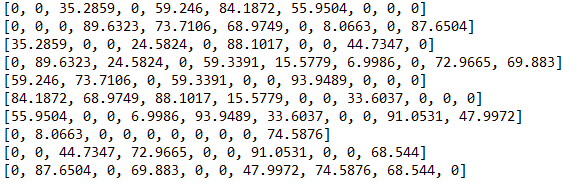
\includegraphics[width=\columnwidth]{assets/graph.png}
    \caption{Example graph of ten vertices utilizing random node deletion in an adjacency matrix}
    \label{fig:example_graph}
\end{figure}

The Traveling Salesman problem is an NP-Hard problem. Exact solutions to the
problem are feasible from a variety of proven conventional algorithms. Of
course, a brute force exhaustive search will yield an optimal path for the
Traveling Salesman, given its time complexity this method will only work on
small graphs. Trying all the permutations would lie in the polynomial factor of
O(n!). Better exact solutions such as Held-Karp, branch and bound,
cutting-plane, and dynamic programming often yield a slightly better result with
a solution to the problem in time O(n\textsuperscript{n}). In worse case
scenarios depending on the graph environment, these solutions are no better than
an exhaustive search. We have included an exhaustive search and an
implementation of the branch and bound algorithm to compete with our proposed
approach at an optimal solution to the Traveling Salesman problem that can be
seen in our results and analysis section. Because the Genetic Hill Climber is a
heuristic solution, it is only possible to provide an approximate solution.
These suboptimal algorithms deliver approximated solutions in a reasonable time
greatly reduced from O(n!) or even eclipsing the time of established exact
algorithm’s O(n\textsuperscript{n}) time. We believe that this type of approach
is appropriate once the graph sizes enlarge to a point where the earlier
mentioned exact solutions would be rendered useless.

\section{Solution}
The solution that is outlined here includes two major concepts, Hill Climbing
and Genetic algorithms. Both are heuristic search techniques used to commonly
solve combinatorial optimization problems. Individually they are both frequently
used for solving the Traveling Salesperson problem. However, the most effective
and tested approaches currently used are neither of these. Those solutions
include Cutting-Plane, Simulated Annealing, Branch and Cut to name a few. As
such, the two algorithms have lost the focus of researchers attempting to
optimize the Traveling Salesman problem. For this reason, these two algorithms
will be the focus of this solution.

A Hill Climbing algorithm is one that uses a state space model to traverse a
problem incrementally through taking steps that minimize cost of the overall
solution. In the simplest form, this is a greedy technique. Where the algorithm
simply evaluates all steps from its current state, and chooses that which
satisfies some cost function the best. There are common improvements on this
principle, one of which is a Stochastic Hill Climber. This is a hill climber
that may not choose the next state that satisfies the cost function the best.
Depending on the implementation this can vary. Some common ways to implement
this model are to choose a random state that improves the current state or has
higher probabilities for choosing better moves than worse ones. It is worth
noting that if you are familiar with Simulated Annealing, this differs in that
the likelihood of accepting a bad move according to the cost function does not
change over time.

A Genetic Algorithm is any algorithm that uses a common set of principles
derived from the theory of evolution. Given a population of potential solutions,
assess each according to some function. Then create a new population of
potential solutions derived in some form from the solutions in the previous
population that satisfy the given function the best. Complex implementations of
this algorithm will include two additional functions, crossover, and mutations.
Crossover is as it is in conventional genetics, in this case combining random
parts of two solutions in the population to create a new solution for the next
population. Mutations would be introducing new random parts of the solution to a
new one regardless of what is reflected in the ‘parent’ solutions. Over each
generation in a Genetic Algorithm, the best individuals of each generation will
approach the best solution.

The concept for this implementation is that when the problem consists of a
complex, large, non-complete graph the starting position of a hill climber can
widely influence the final solution. Here, the starting position of the hill
climber is being optimized by a Genetic algorithm. Each generation introduces
new instances of hill climbers to the population whose starting position is
based relative to the best individual hill climbers of previous populations.

Both the hill climbing individuals and the Genetic algorithm instantiating them
have a stochastic element. The hill climbers have a fixed chance of taking a
random move from the available moves from their current position on the graph.
This allows them to potentially make it over a local maxima and wider variance
of paths from the same or similar starting positions of the previous fittest
individual hill climbers. Within the genetic portion of the algorithm, there is
the additional layer of stochastism by which the creation of a generation has a
fixed chance of implementing a new hill climber from a completely random point
on the graph, this is the mutation portion of the Genetic algorithm. This allows
the algorithm to constantly test completely new areas of the graph that it had
not considered before in the creation of climber.

There are several variables involved in addition to the input for the solution.
There is the number of generations that will be used (G) and the number of
individuals in each population (P). The input size can be measured as the number
of nodes within the graph that represents the state space of the problem. Given
this, the time complexity of the implementation of the algorithm described can
be expressed as the following. Note that the approximation is the value obtained
in the testing shown in the next section of the paper.

\begin{figure}
    \[ \sum_{k=1}^{G}\sum_{j=1}^{P}\sum_{i=1}^{N}\sum_{q=1}^{N}1 = 0\Big(G\times
        P \times N\textsuperscript{2}\Big) \approx
        O\Bigg(N\textsuperscript{3}\Bigg) \]
    \caption{Theoretical time complexity of the Genetic Hill Climber with inputs being number of Generations, Populations, and Nodes}
\end{figure}

\section{Perfromance Evaulation}
Firstly, before analysis of our developed Genetic Hill Climber, the results of
the conventional approaches to the Traveling Salesman problem should be looked
at first. Using our graph environments that were created and discussed earlier
in the problem definition section, we were unable to obtain optimal solutions to
the graphs once the number of nodes passed 15. Graphs of size 20 vertices and
higher, no optimal solutions were able to be found. This could be attributed to
the circumstances of our testing machine. In attempts to find the optimal
solution either using an exhaustive search or the Branch and Bound algorithm,
our machine ran for several hours until an abort was conducted due to a
limitation of memory. For the graph of 15 nodes, utilizing an exhaustive search,
the solution was found after a surplus of many hours though the exact runtime
was not recorded. For the Branch and Bound algorithm running on a graph of 15
nodes, the run time was a $339.85$ seconds. Additionally, it must be pointed out
that the solutions that were obtained via branch and bound were not as optimal
and exact in comparison to the exhaustive search. Our accuracy metric for
evaluating these solutions uses a fitness definition that can be defined as the
total amount of length found in the circuit divided by the total amount of
nodes. This could be due to our implementation of the Branch of Bound algorithm
where certain branches are excluded from the optimal solution due to the graphs
not being complete. These dead ends in the graph could result in the algorithm
failing to find the global maximum. This can be seen where only the optimal
fitness is equal for the graph of five nodes. Once the graph increases to a size
of ten and 15 nodes, the fitness differs between the branch and bound algorithm
compared exhaustive search.

These results show that these traditional solutions to the Traveling Salesman
problem are not reliable once a graph scales to a certain size. It is extremely
easy for real world applications to require more than 15 nodes. Once again it
must be emphasized that in this situation the limiting factor would be our
machine when conducting these tests. This data and conclusion can be referenced
in table \ref{table:branch_and_bound_table} where there are blanks in columns
one through five from a lack of data that could not be obtained for graphs of
nodes greater than 15. Attempting to fit the Branch and Bound algorithm on a
time complexity chart shows poorly without our test data of three points. As
can be seen in figure \ref{fig:branch_and_bound_time_complexity}, due to
scaling, even if a fourth point were to be obtained with an X-axis of 20 nodes,
the line of best fit for a graph of n\textsuperscript{n} would project to be a
near vertical line.

\begin{table}[h]
    \setlength\tabcolsep{2pt}
    \centering
    \begin{tabular}{c|c|c|c|c}
    \multicolumn{5}{c}{\textbf{Branch and Bound}}                                                   \\
    \hline
    \text{Nodes} & \text{Time(seconds)} & \text{Fitness} & \text{Optimal Fitness} & \text{\% Error} \\
    \hline
    5            & $0.0004961$          & $74.08426$     & $74.08426$             & $0$             \\
    10           & $0.0168638$          & $57.99643$     & $45.86036$             & $0.26463$       \\
    15           & $339.8524076$        & $50.03704$     & $18.30926$             & $1.73288$       \\
    20           & -                    & -              & -                      & -               \\
    25           & -                    & -              & -                      & -               \\
    50           & -                    & -              & -                      & -               \\
    75           & -                    & -              & -                      & -               \\
    100          & -                    & -              & -                      & -               \\
    125          & -                    & -              & -                      & -               \\
    150          & -                    & -              & -                      & -               \\
    175          & -                    & -              & -                      & -               \\
    200          & -                    & -              & -                      & -               \\
    300          & -                    & -              & -                      & -               \\
    400          & -                    & -              & -                      & -               \\
    500          & -                    & -              & -                      & -               \\
\end{tabular}


    \caption{Runtimes and fitness of the Branch and Bound algorith in comparison to the optimal fitness found in an exhaustive search}
    \label{table:branch_and_bound_table}
\end{table}

\begin{figure}[h]
    \centering
    \textbf{Branch and Bound Time Complexity}
    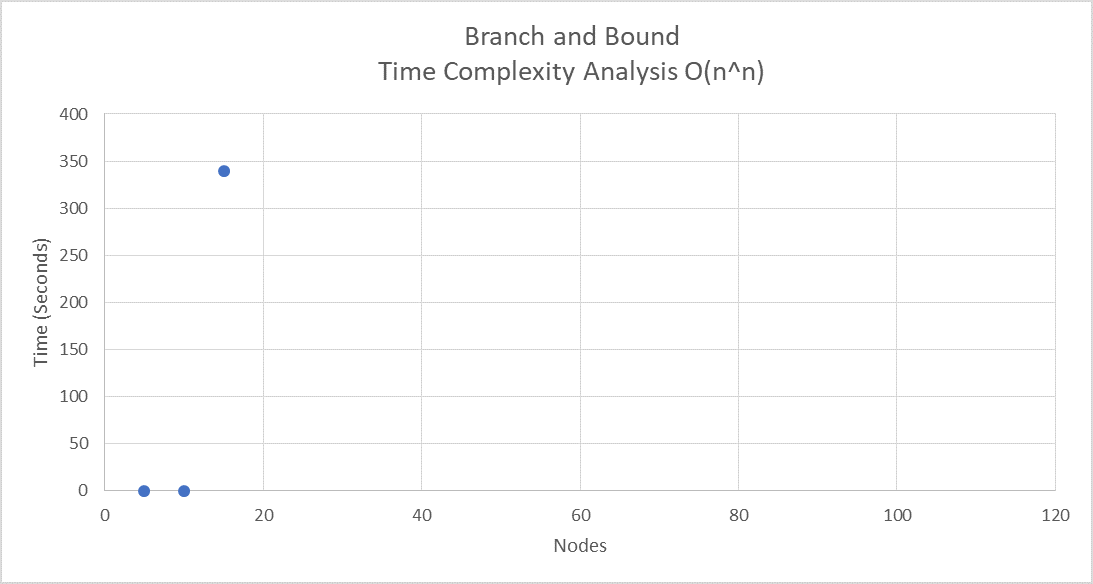
\includegraphics[width=\columnwidth]{assets/branch_and_bound_time_complexity.png}
    \caption{Time complexity of the Branch and Bound algorithm using limited runtime data}
    \label{fig:branch_and_bound_time_complexity}
\end{figure}

Next, upon examination, our Stochastic Hillclimber, which eventually will be
developed as a Genetic Hill Climber, provided us with appalling results. The
Stochastic Hill Climber was able to quickly traverse the graphs and provide
solutions where the other conventional methods were not. At one end of the
spectrum with a graph of five vertices, it was able to obtain the same optimal
fitness as both the Branch and Bound algorithm as well as the exhaustive search
with a fitness of $74.08426$. Although this is not much of an achievement given
the small size of the graph. The run times were comparable as well within ten
thousandths of a second. These times were kept until a graph of 50 nodes was
introduced where the hill climber took a thousandth of a second to calculate a
heuristic solution. These quick times continued all the way to the other end of
the spectrum with a $0.28519$ second run time for a graph of 500 nodes. These
data values can be seen in table \ref{table:hill_climber_table}. As
mathematically defined in the solutions section, this a glaring obvious
difference between a time complexity of O(n\textsuperscript{n}) and a time
complexity of O(n\textsuperscript{2}). The Stochastic Hill Climber time
complexity chart can be seen in figure \ref{fig:hill_climber}. Despite these
quick times, due to our limitations of the other conventional approach, we are
unsure of how our fitness that was obtained from the Stochastic Hill Climber
compares to an optimal fitness. In other words, even though a solution was
generated, we are unsure of how accurate and optimal this solution is. This just
goes to show the complexity of the NP-Hard problem that is the Traveling
Salesman.

\begin{table}[h]
    \setlength\tabcolsep{2pt}
    \centering
    \begin{tabular}{c|c|c|c|c}
    \multicolumn{5}{c}{\textbf{Stochastic Hill Climber}}                                            \\
    \hline
    \text{Nodes} & \text{Time(seconds)} & \text{Fitness} & \text{Optimal Fitness} & \text{\% Error} \\
    \hline
    5            & $0.0004804$          & $74.08426$     & $74.08426$             & $0$             \\
    10           & $0.0004966$          & $55.173$       & $45.86036$             & $0.20299$       \\
    15           & $0.0004954$          & $28.21844$     & $18.30926$             & $0.54121$       \\
    20           & $0.0009851$          & $21.96413$     & -                      & -               \\
    25           & $0.0004961$          & $23.15343$     & -                      & -               \\
    50           & $0.0014879$          & $18.45314$     & -                      & -               \\
    75           & $0.0034711$          & $13.36534$     & -                      & -               \\
    100          & $0.0064475$          & $13.24880$     & -                      & -               \\
    125          & $0.0089280$          & $14.08632$     & -                      & -               \\
    150          & $0.0143837$          & $11.71591$     & -                      & -               \\
    175          & $0.0183513$          & $9.423754$     & -                      & -               \\
    200          & $0.0247995$          & $11.53126$     & -                      & -               \\
    300          & $0.0709278$          & $12.72170$     & -                      & -               \\
    400          & $0.1547515$          & $7.936304$     & -                      & -               \\
    500          & $0.2851998$          & $9.040675$     & -                      & -               \\
\end{tabular}
    \caption{Run times of the Stochastic Hill Climber and obtained Fitness}
    \label{table:hill_climber_table}
\end{table}


\begin{figure}[h]
    \centering
    \textbf{Stochastic Hill Climber Time Complexity}
    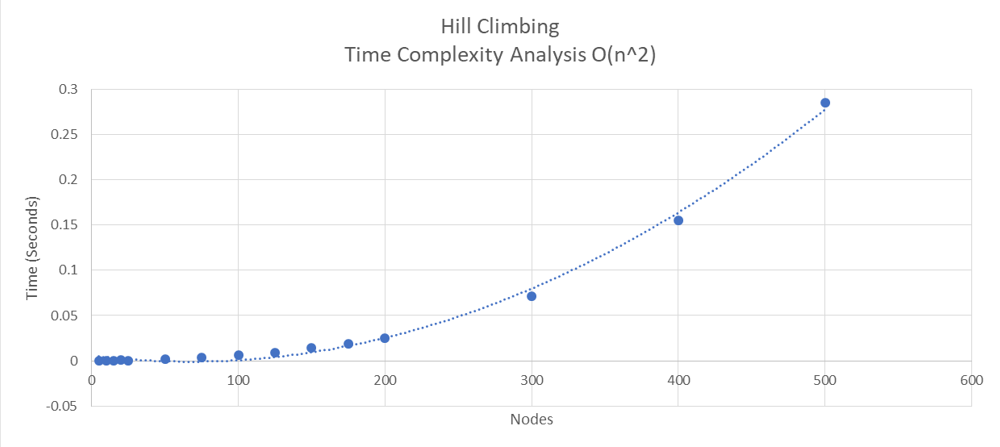
\includegraphics[width=\columnwidth]{assets/hill_climber.png}
    \caption{Time complexity of the Stochastic Hill Climber using our run time data}
    \label{fig:hill_climber}
\end{figure}

Immediately looking at the data for the developed Genetic Hill Climber, run
times are drastically higher compared to the Stochastic Hill Climber. For the
graph of five nodes, the Genetic Hill Climber took approximately 250 times
longer compared to the Stochastic Hill Climber. Once the graphs enlargened to a
size of 500, the Stochastic Hill Climber had a faster run time by a factor of
nearly 100. We deliberately decided to exclude a runtime graph to compare these
two algorithms due to the vast differences in performance. Using our data, this
type of chart would show the Genetic Hill Climber as exponential while the
Stochastic Hill Climber would appear linear despite it being
O(n\textsuperscript{2}). However, there is an included graph which can show the
estimates of basic operations per given number of nodes with these two
algorithms side by side (fig. \ref{fig:hc_vs_ghc}). This estimate of using theoretical
number of computations more closely resembles how these two graphs should look
when compared with one another. However, there is still a misleading linear type
of line and exponential line can clearly be seen. Table
\ref{table:ghc_vs_hc_table} shows these run times side by side where the
comparison can be more easily seen with the Stochastic Hill Climber being much
quicker compared to the slower Genetic Hill Climbing algorithm.

\begin{table}[h]
    \setlength\tabcolsep{2pt}
    \centering
    \begin{tabular}{c|c|c}
    \multicolumn{3}{c}{\textbf{Genetic Hill Climber}}      \\
    \multicolumn{3}{c}{\textbf{Vs.}}                       \\
    \multicolumn{3}{c}{\textbf{Stochastic Hill Climber}}   \\
    \multicolumn{3}{c}{\textbf{(seconds)}}                 \\
    \hline
    Nodes & Genetic Hill Climber & Stochastic Hill Climber \\
    \hline
    5     & $0.10316$            & $0.00048$               \\
    10    & $0.11755$            & $0.00049$               \\
    15    & $0.12796$            & $0.00049$               \\
    20    & $0.14284$            & $0.00098$               \\
    25    & $0.19344$            & $0.00049$               \\
    50    & $0.33231$            & $0.00148$               \\
    75    & $0.57833$            & $0.00347$               \\
    100   & $0.89924$            & $0.00644$               \\
    125   & $1.32828$            & $0.00892$               \\
    150   & $1.77617$            & $0.01438$               \\
    175   & $2.52414$            & $0.01835$               \\
    200   & $3.27260$            & $0.02479$               \\
    300   & $8.49250$            & $0.07092$               \\
    400   & $16.37443$           & $0.15475$               \\
    500   & $30.20190$           & $0.28519$               \\
\end{tabular}
    \caption{Run times between the Genetic Hill Climber and the Stochastic Hill Climber}
    \label{table:ghc_vs_hc_table}
\end{table}

\begin{figure}[h]
    \centering
    \textbf{Computed Time Complexity of Stochastic Hill Climber vs. Genetic Hill Climber}
    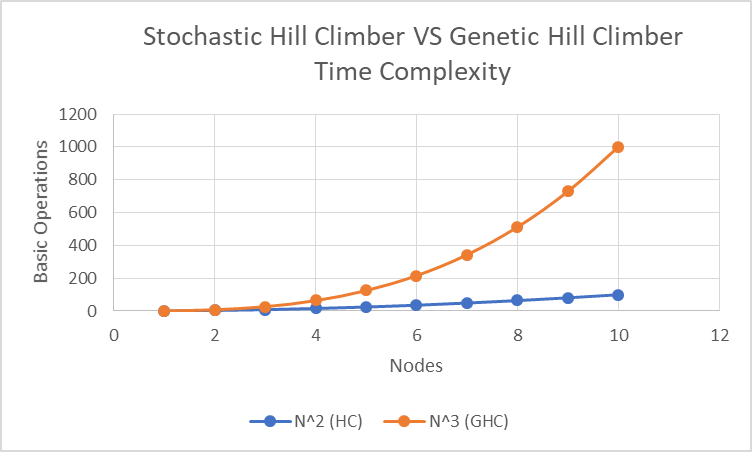
\includegraphics[width=\columnwidth]{assets/hc_vs_ghc.png}
    \caption{Computed time complexity of our Stochastic Hill Climber compared to our Genetic Hill Climber using theoretical mathematical data}
    \label{fig:hc_vs_ghc}
\end{figure}

As for fidelity to the solutions, the Genetic Hill Climber was able to best the
Stochastic Hill Climber in every scenario except for the case of a graph with
five nodes, as can be seen in table \ref{table:hc_vs_ghc_fitness} where they
managed to obtain the same optimal fitness. This is a strong indication that our
Genetic Hill Climber would be able to further find more optimal solutions with
an even larger graph than the sizes than presented. It must be noted that our
variation of the Genetic Hill Climber started with a population of ten
individuals propagating within ten generations. After this initial phase of
testing, we were able to generate the test data that is shown above and within
the variance chart as well as below in the standalone Genetic Hill Climbing
data. Since we were able to best the Stochastic Hill Climber early on, we did
not further progress to see the optimal number of populations and generations as
our initial proposal was to simply best a basic Hill Climber in fitness. It can
safely be said that the Genetic Hill Climber exchanges time complexity for
accuracy. Obtaining better results with a lower fitness than the Stochastic Hill
Climber, however the Genetic Hill Climber slowed down a large amount. The
standalone data for the Genetic Hill Climber follows below.

\begin{table}[h]
    \centering
    \begin{tabular}{c|c|c}
    \multicolumn{3}{c}{\textbf{Genetic Hill Climber}}      \\
    \multicolumn{3}{c}{\textbf{Vs.}}                       \\
    \multicolumn{3}{c}{\textbf{Stochastic Hill Climber}}   \\
    \multicolumn{3}{c}{\textbf{Fitness}}                   \\
    \hline
    Nodes & Genetic Hill Climber & Stochastic Hill Climber \\
    \hline
    5     & $74.08426$           & $74.08426$              \\
    10    & $45.93808$           & $55.17$                 \\
    15    & $18.84321$           & $28.21844$              \\
    20    & $21.96413$           & $21.96413$              \\
    25    & $18.89756$           & $23.15343$              \\
    50    & $16.10445$           & $18.45314$              \\
    75    & $12.43940$           & $13.36534$              \\
    100   & $11.41996$           & $13.24880$              \\
    125   & $8.60325$            & $14.08632$              \\
    150   & $8.61659$            & $11.71591$              \\
    175   & $8.25562$            & $9.42375$               \\
    200   & $6.89503$            & $11.53126$              \\
    300   & $8.02294$            & $12.72170$              \\
    400   & $7.29255$            & $7.93630$               \\
    500   & $7.09442$            & $9.04067$               \\
\end{tabular}
    \caption{Fitness of Genetic Hill Climber vs. Stochastic Hill Climber}
    \label{table:hc_vs_ghc_fitness}
\end{table}

\begin{figure}[h]
    \centering
    \textbf{Genetic Hill Climber Time Complexity}
    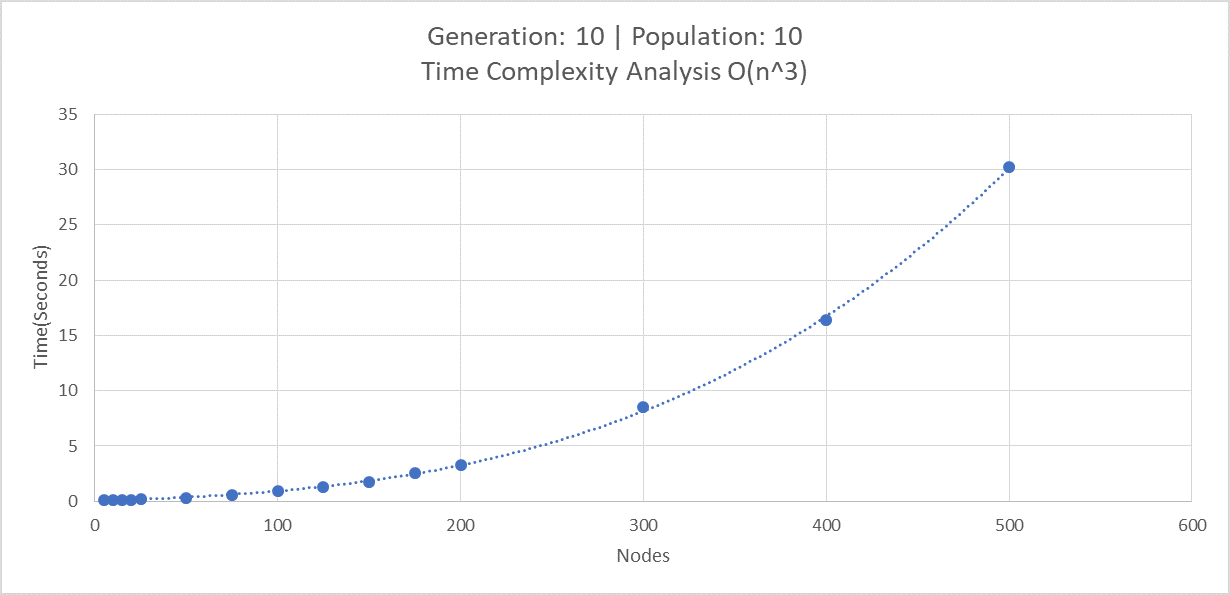
\includegraphics[width=\columnwidth]{assets/ghc_graph.png}
    \caption{The Genetic Hill Climber time complexity can be seen as
        O(n\textsuperscript{3}) taking longer run times compared to the
        Stochastic Hill Climber}
    \label{fig:ghc_timecomplexity}
\end{figure}

\begin{table}[h]
    \centering
    \begin{tabular}{c|c|c|c|c}
    \multicolumn{5}{c}{\textbf{Genetic Hill Climber}}                                               \\
    \hline
    \text{Nodes} & \text{Time(seconds)} & \text{Fitness} & \text{Optimal Fitness} & \text{\% Error} \\
    \hline
    5            & $0.10316$            & $74.08426$     & $74.08426$             & $0$             \\
    10           & $0.11755$            & $45.93808$     & $45.86036$             & $0.20299$       \\
    15           & $0.12796$            & $18.84321$     & $18.30926$             & $0.54121$       \\
    20           & $0.14284$            & $21.96413$     & -                      & -               \\
    25           & $0.19344$            & $18.89756$     & -                      & -               \\
    50           & $0.33231$            & $16.10445$     & -                      & -               \\
    75           & $0.57833$            & $12.43940$     & -                      & -               \\
    100          & $0.89924$            & $11.41996$     & -                      & -               \\
    125          & $1.32828$            & $8.60325$      & -                      & -               \\
    150          & $1.77617$            & $8.61659$      & -                      & -               \\
    175          & $2.52414$            & $8.255624$     & -                      & -               \\
    200          & $3.27260$            & $6.89503$      & -                      & -               \\
    300          & $8.49250$            & $8.02294$      & -                      & -               \\
    400          & $16.37443$           & $7.29255$      & -                      & -               \\
    500          & $30.20190$           & $7.09442$      & -                      & -               \\
\end{tabular}
    \caption{Run time data of the Genetic Hill Climber and obtained fitness}
    \label{table:ghc_table}
\end{table}

\begin{figure}[h]
    \centering
    \textbf{Stochastic Hill Climber VS Genetic Hill Climber Variance from Optimal Fitness}
    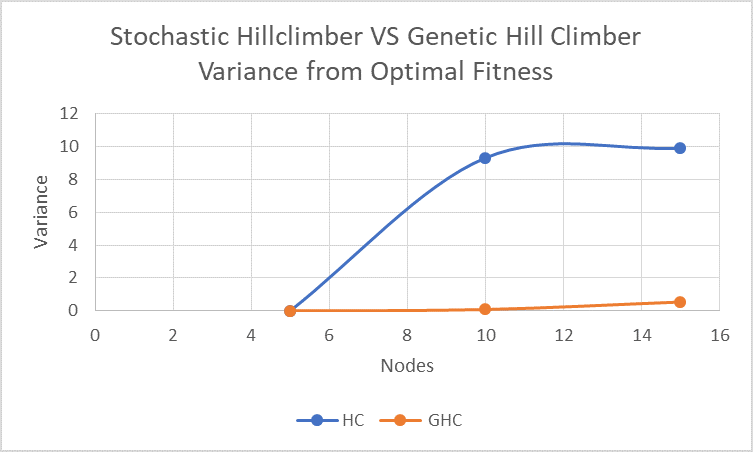
\includegraphics[width=\columnwidth]{assets/hc_vs_ghc_variance.png}
    \caption{This graph shows the variance of the two algorithms from the optimal fitness. Note: limited graph data}
    \label{fig:variance}
\end{figure}

\clearpage
\section{Prognosis}
All objectives that were planned within the initial start of this project were
completed at its conclusion. No difficulties were encountered regarding
algorithm design and analysis, however we encountered difficulties with
development as the technologies used were unfamiliar.

Our developed Genetic Hill Climbing algorithm was able to obtain suboptimal
solutions to the Traveling Salesman problem while conventional approaches were
not able to do so. The algorithm yielded solutions, however the optimality of
these are unverified because we were unable to obtain exact solutions for our
set of large graphs. Despite this, it should be seen on a positive note that any
solution could be interpreted as better than no solutions.

Through our runtimes, we were able to conclude that the runtime analysis does
not reflect the theoretical time complexity disused in the solutions section.
The graphs and data obtained allowed us to approximate the time complexity and
number of basic operations. Perhaps due to the limited number of generations and
populations, these variables in the time complexity equation only seemed to
result as a single n input instead of an input of n\textsuperscript{n}. As
mentioned earlier, we did not proceed with further testing and optimization to
find the optimal number of generations and populations. Further alteration of
the algorithm's parameters could affect run times and obtained fitness which we
did not test. With that being said, we believe our solution is unable to compete
with other forefront heuristic solutions without improvements. This is further
expanded upon later.

\section{Conclusion and Future Work}
In closing, it is clear that a lot of improvements would be necessary to be made
for this to compete with other heuristic algorithms used for solving the
Traveling Salesman problem. The data has shown that this solution does allow for
the generation of good sub-optimal solutions in an efficient manner compared to
conventional approaches. At best any answer is better than no answer. It is also
possible this methodology might be more effective for other combinatorial
optimization problems.

The representation used for the Traveling Salesman Problem in this
implementation was an adjacency matrix as described in a previous section.
Implementing the representation as an adjacency list would have significantly
cut down on the overhead of the entire implementation. Quicker run times could
have potentially been obtained. It may also improve the time complexity to
create graphs allowing for more testing data of larger sizes. Creating Graphs of
large sizes took a significant amount of time.

In the future, modifying the algorithm such that the size of the population and
the number of generations is determined by the complexity of the problem might
allow for further time reduction. Similarly, the algorithm could be modified to
continue creating new generations until the cost function yields a particular
level of optimality. This would allow the algorithm to end sooner if a near goal
state that meets the needs of the problem has already been found.

If instead of allowing the hill climbers in each generation of our algorithm run
to completion, there was an evaluation function to end and replace hill climbers
that have a low probability of improving the next generation, a large amount of
run time could be avoided. Similarly, if the population existed with hill
climbers that are all at various stages of completion, there would be only one
continuous population through each generation. Though this might not make the
complexity of the algorithm any different, it would improve the ease of
implementing some of the earlier suggested improvements to dynamic set the
population size and number of hill climbers created. In short, these
improvements would allow for the same amount of compute time to be spent on
solutions with a higher probability of improving upon the best solution.

Similarly, to Simulated Annealing, it would be possible and more optimal to
change the level of stochastisim as the algorithm progressively gets closer to
the optimal solution. During the beginning, allowing more movement around the
graph for starting positions would result in finding the way around large global
minimums early. Furthermore, it would also be possible to implement this design
using a population of Simulated Annealing Climbers, though it is unsure if this
would be any improvement.

\bibliographystyle{ACM-Reference-Format}
\bibliography{report}

\end{document}
\endinput
